\documentclass[9pt,aspectratio=169,xcolor=table]{beamer}

%~~~~~~~~~~~~~~~~~~~~~~~~~~~~~~~~~~~~~~~~~~~~~~~~~~~~~~~~~~~~~~~~~~~~~~~~~~~~~~
% Use roboto Font (recommended)
\usepackage[sfdefault]{roboto}
\usepackage[utf8]{inputenc}
\usepackage[T1]{fontenc}
%~~~~~~~~~~~~~~~~~~~~~~~~~~~~~~~~~~~~~~~~~~~~~~~~~~~~~~~~~~~~~~~~~~~~~~~~~~~~~~

%~~~~~~~~~~~~~~~~~~~~~~~~~~~~~~~~~~~~~~~~~~~~~~~~~~~~~~~~~~~~~~~~~~~~~~~~~~~~~~
% Define where theme files are located. ('/styles')
\usepackage{styles/fluxmacros}
\usefolder{styles}
% Use Flux theme v0.1 beta
% Available style: asphalt, blue, red, green, gray
\usetheme[style=gray]{flux}
%~~~~~~~~~~~~~~~~~~~~~~~~~~~~~~~~~~~~~~~~~~~~~~~~~~~~~~~~~~~~~~~~~~~~~~~~~~~~~~

%~~~~~~~~~~~~~~~~~~~~~~~~~~~~~~~~~~~~~~~~~~~~~~~~~~~~~~~~~~~~~~~~~~~~~~~~~~~~~~
% Extra packages
\usepackage{booktabs}
\usepackage{colortbl}
\usepackage{ragged2e}
\usepackage{amssymb}
\usepackage{multirow}
\usepackage{tikz}
\usetikzlibrary{arrows.meta, positioning, fit, backgrounds, calc, decorations.pathreplacing, shapes.geometric}
\setbeamertemplate{itemize items}[square]
\usepackage[scaled=.8]{beramono}
\usepackage{listings}
\usepackage{styles/lstlangarm}
\usepackage{array}
\definecolor{bgcolor}{HTML}{F2E9E9}
% lstlangarm.sty references \color{mauve} for string literals but never defines
% it -- only fires when a listing contains a string. Define it here.
\definecolor{mauve}{rgb}{0.58,0,0.82}
% lstlangarm's C style sets commentstyle=green!20, which is unreadable on the
% pink listing background. Darken it globally.
\lstset{commentstyle=\color{green!45!black}}
% ragged-right fixed-width column -- must be defined in the preamble, never
% inside a frame (\newcolumntype's #1 breaks beamer's frame scanner)
\newcolumntype{R}[1]{>{\RaggedRight\arraybackslash}p{#1}}
%~~~~~~~~~~~~~~~~~~~~~~~~~~~~~~~~~~~~~~~~~~~~~~~~~~~~~~~~~~~~~~~~~~~~~~~~~~~~~~
% Table striping: odd rows white, even rows very light gray.
% Needs \documentclass[...,xcolor=table]{beamer} (beamer loads xcolor itself,
% so the option must go on the class, not \usepackage).
\definecolor{stripe}{gray}{0.94}
% \striped makes body rows alternate white, gray, white, ... starting white.
% \rowcolors counts from the first coloured body row; the header is not counted.
\newcommand{\striped}{\rowcolors{1}{white}{stripe}}
%~~~~~~~~~~~~~~~~~~~~~~~~~~~~~~~~~~~~~~~~~~~~~~~~~~~~~~~~~~~~~~~~~~~~~~~~~~~~~~

%~~~~~~~~~~~~~~~~~~~~~~~~~~~~~~~~~~~~~~~~~~~~~~~~~~~~~~~~~~~~~~~~~~~~~~~~~~~~~~
% TikZ block styles -- matches ch1/ch2
% Colour variables are named identically in the book's stm32primer.tex, so any
% tikzpicture using only the \tikzset{...} styles below can be copied verbatim
% between slides and book. Only the \definecolor/\colorlet VALUES differ: the
% book is printed, so it keeps every stroke pure black with muted fills. These
% slides are projected, so both fill AND stroke are bright and saturated to
% grab attention -- see stm32primer.tex for the print palette.
\definecolor{blkfill}{HTML}{DCEBFF}
\definecolor{blkline}{HTML}{1565C0}
\definecolor{accentfill}{HTML}{FFE0B2}
\definecolor{accentline}{HTML}{E65100}
\definecolor{memfill}{HTML}{DFF5DA}
\definecolor{memline}{HTML}{2E7D32}
\definecolor{cellfill}{HTML}{FFFFFF}
\definecolor{cellline}{HTML}{424242}
\definecolor{bitmaskfill}{HTML}{DCEBFF}
\definecolor{bitmaskline}{HTML}{1565C0}
\definecolor{bithitfill}{HTML}{FFE0B2}
\definecolor{bithitline}{HTML}{E65100}
\tikzset{
  blk/.style   = {rectangle, rounded corners=2pt, draw=blkline, fill=blkfill,
                  thick, align=center, font=\small, minimum height=9mm, inner sep=3pt},
  cpublk/.style= {rectangle, rounded corners=2pt, draw=accentline, fill=accentfill,
                  thick, align=center, font=\small\bfseries, minimum height=9mm, inner sep=3pt},
  memblk/.style= {rectangle, rounded corners=2pt, draw=memline, fill=memfill,
                  thick, align=center, font=\small, minimum height=9mm, inner sep=3pt},
  cell/.style  = {rectangle, draw=cellline, fill=cellfill, align=center,
                  font=\small\ttfamily, minimum height=7mm, inner sep=2pt},
  lbl/.style   = {font=\scriptsize, text=Gray},
  flow/.style  = {-{Stealth[length=2mm]}, thick, draw=blkline},
  busline/.style={thick, draw=cellline},
}
% NOTE (theme quirks -- all fail SILENTLY, always page through the PDF):
%  - a second \\ inside a nested {...} group in a TikZ node breaks parsing
%  - {\small ...} wrapped around a nested itemize eats the frame title + list
%  - \usebeamercolor on a [plain] frame falls through to an unstyled default
%  - \newcolumntype inside a frame breaks beamer's frame scanner
%  - lstlisting needs \begin{frame}[fragile]
%  - a TikZ picture wider than its column silently overflows into neighbours
%~~~~~~~~~~~~~~~~~~~~~~~~~~~~~~~~~~~~~~~~~~~~~~~~~~~~~~~~~~~~~~~~~~~~~~~~~~~~~~

%%%%%%%%%%%%%%%%%%%%%%%%%%%%%%%%%%%
%% BEGIN CONDITIONAL COMPILATION %%
%%%%%%%%%%%%%%%%%%%%%%%%%%%%%%%%%%%
\newif\ifwebex
%\webextrue % uncomment to generate section separator
\ifwebex
\AtBeginSection[]{
  \begin{frame}
  \vfill
  \centering
  \begin{beamercolorbox}[sep=8pt,center,shadow=true,rounded=true]{title}
    \usebeamerfont{title}\insertsectionhead\par%
  \end{beamercolorbox}
  \vfill
  \end{frame}
}
\else
\AtBeginSection[]
{
{
    \setbeamercolor{background canvas}{bg=yellow!10}
    \begin{frame}[plain]
        \frametitle{Table of Contents}
        \tableofcontents[currentsection]
    \end{frame}
}
}
\fi
%%%%%%%%%%%%%%%%%%%%%%%%%%%%%%%%%%%
%% END CONDITIONAL COMPILATION   %%
%%%%%%%%%%%%%%%%%%%%%%%%%%%%%%%%%%%

%~~~~~~~~~~~~~~~~~~~~~~~~~~~~~~~~~~~~~~~~~~~~~~~~~~~~~~~~~~~~~~~~~~~~~~~~~~~~~~
% Information
\title{UART Communication}
\subtitle{\emph{Introduction to ARM Cortex-M Microprocessors} --- Chapter 12}
\author{Mun\'{i}m Zabidi}
\institute{\color{primary}Faculty of Electrical Engineering, Universiti Teknologi Malaysia}
\date{\today}
\titlegraphic{assets/logoutmwhite.png}
%~~~~~~~~~~~~~~~~~~~~~~~~~~~~~~~~~~~~~~~~~~~~~~~~~~~~~~~~~~~~~~~~~~~~~~~~~~~~~~

\begin{document}

\titlepage

\begin{frame}{Table of Contents}
    \tableofcontents
\end{frame}

%===============================================================================
\section{Why This Matters}
%===============================================================================

\begin{frame}{Why This Chapter Matters}
    \leavevmode
    Until now, seeing what your program is doing has required a debugger and a breakpoint. The \alert{UART} (Universal Asynchronous Receiver/Transmitter) changes that: with a few lines of code the microcontroller can print to a terminal on your PC. That makes it the single most valuable debugging tool in embedded development --- and it is also how the device talks to GPS modules, Bluetooth radios, and industrial instruments. From this chapter onward, you should use it in every program you write.
\end{frame}

\begin{frame}{Objectives}
    \leavevmode
    {\small After completing this chapter, you should be able to:}

    \vspace{2mm}
    {\small
    \begin{enumerate}\itemsep2pt
        \item Contrast parallel with serial and synchronous with asynchronous transmission.
        \item Describe every field of a UART frame and state the purpose of the start and stop bits.
        \item Calculate the \texttt{BRR} register value for any required baud rate.
        \item Configure a USART peripheral and its alternate-function pins.
        \item Transmit and receive characters by polling and by interrupt.
        \item Use UART output as a diagnostic instrument in your own programs.
    \end{enumerate}}
\end{frame}


%===============================================================================
\section{Serial Fundamentals}
%===============================================================================

\begin{frame}{Serial versus Parallel}
    \begin{columns}[T]
    \begin{column}{.48\textwidth}
        \textbf{Serial}
        \begin{itemize}
            \item One bit at a time, over a \alert{single} wire
            \item Efficient over \alert{long distances}
            \item Few pins
        \end{itemize}
    \end{column}
    \begin{column}{.48\textwidth}
        \textbf{Parallel}
        \begin{itemize}
            \item Many bits at once, over \alert{many} wires
            \item Faster over \alert{short distances}
            \item Costs pins and board area
        \end{itemize}
    \end{column}
    \end{columns}

    \vspace{3mm}
    \begin{center}
    \begin{tikzpicture}[x=10mm, y=8mm]
        \node[cpublk, minimum width=20mm] (m1) at (0,0.6) {MCU};
        \node[blk,    minimum width=20mm] (d1) at (5.2,0.6) {device};
        \draw[busline, draw=secondary] (m1) -- node[lbl, above] {1 wire} (d1);
        \node[lbl, anchor=west] at (6.4,0.6) {serial};
        \node[cpublk, minimum width=20mm] (m2) at (0,-0.9) {MCU};
        \node[blk,    minimum width=20mm] (d2) at (5.2,-0.9) {device};
        \foreach \dy in {-0.18,-0.09,0,0.09,0.18}{
            \draw[busline, draw=tertiary] ([yshift=\dy cm]m2.east) -- ([yshift=\dy cm]d2.west);
        }
        \node[lbl, anchor=west] at (6.4,-0.9) {parallel};
    \end{tikzpicture}
    \end{center}

    \vspace{2mm}
    {\small \textbf{Asynchronous} means no shared clock --- so each byte carries
    its own framing. \textbf{Synchronous} adds a clock wire and removes the need
    for both ends to agree on speed in advance.}
\end{frame}

\begin{frame}{Wiring a UART Link: The Crossover}
    \begin{center}
    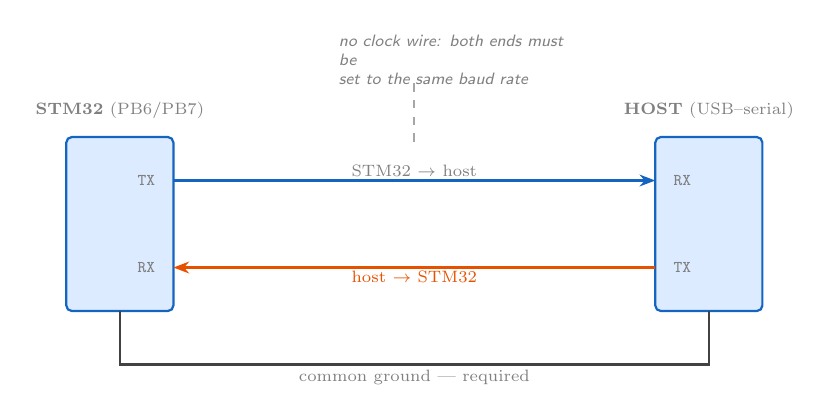
\begin{tikzpicture}[scale=0.85, every node/.style={transform shape}]

    % Device bodies
    \draw[draw=blkline, fill=blkfill, thick, rounded corners=2pt]
        (-1.6,-1.3) rectangle (0,1.3);
    \draw[draw=blkline, fill=blkfill, thick, rounded corners=2pt]
        (7.2,-1.3) rectangle (8.8,1.3);
    \node[lbl] at (-0.8,1.7) {\textbf{STM32} (PB6/PB7)};
    \node[lbl] at (8.0,1.7)  {\textbf{HOST} (USB--serial)};

    % Pin labels
    \node[lbl, anchor=east, font=\scriptsize\ttfamily] at (-0.15,0.65)  {TX};
    \node[lbl, anchor=east, font=\scriptsize\ttfamily] at (-0.15,-0.65) {RX};
    \node[lbl, anchor=west, font=\scriptsize\ttfamily] at (7.35,0.65)  {RX};
    \node[lbl, anchor=west, font=\scriptsize\ttfamily] at (7.35,-0.65) {TX};

    % The crossover: each TX drives the other end's RX
    \draw[flow] (0,0.65) -- (7.2,0.65);
    \draw[flow, draw=accentline] (7.2,-0.65) -- (0,-0.65);

    \node[lbl, above, inner sep=1.5pt] at (3.6,0.65) {STM32 $\rightarrow$ host};
    \node[lbl, below, inner sep=1.5pt, text=accentline] at (3.6,-0.65) {host $\rightarrow$ STM32};

    % Common ground
    \draw[busline] (-0.8,-1.3) -- (-0.8,-2.1) -- (8.0,-2.1) -- (8.0,-1.3);
    \node[lbl, below, inner sep=2pt] at (3.6,-2.1) {common ground --- required};

    % No clock: the defining contrast with the synchronous buses
    \node[lbl, anchor=west, text width=34mm, font=\sffamily\scriptsize\itshape]
         at (2.35,2.45) {no clock wire: both ends must be\\set to the same baud rate};
    \draw[busline, dashed, draw=black!35] (3.6,2.1) -- (3.6,1.15);

    \end{tikzpicture}
    \end{center}

    \vspace{1mm}
    {\small A UART link is three wires. Each device's \alert{TX drives the other's
    RX} --- the crossover --- and both must share a \alert{common ground}. There is
    no clock line, which is why both ends must independently agree on the baud rate.}
\end{frame}

\begin{frame}{The UART Frame}
    \begin{center}
    \begin{tikzpicture}[x=10mm, y=9mm]
        \node[cell, minimum width=11mm, draw=primary, fill=primary!12] (s) at (0,0) {start};
        \foreach \i in {0,...,7}{
            \pgfmathsetmacro{\x}{1.15+\i*0.95}
            \node[cell, minimum width=9mm] at (\x,0) {D\i};
        }
        \node[cell, minimum width=11mm, draw=tertiary, fill=tertiary!12] (p) at (9.0,0) {par};
        \node[cell, minimum width=11mm, draw=primary, fill=primary!12] (e) at (10.3,0) {stop};
        \node[lbl, anchor=north, align=center] at (0,-0.55) {always 0\\marks the start};
        \node[lbl, anchor=north, align=center] at (5.2,-0.55) {8 data bits, \alert{LSB first}};
        \node[lbl, anchor=north, align=center] at (9.0,-0.55) {optional};
        \node[lbl, anchor=north, align=center] at (10.3,-0.55) {always 1};
        \node[lbl, anchor=east] at (-0.7,0) {idle = 1};
    \end{tikzpicture}
    \end{center}

    \vspace{4mm}
    \begin{block}{Why asynchronous needs a start bit}
        With no shared clock, the receiver must know \alert{when} a byte begins.
        The line drops from idle-high to low, and the receiver counts bit periods
        from that edge.
    \end{block}

    \vspace{1mm}
    {\small Both ends must agree in advance on \alert{baud rate, data bits, parity
    and stop bits} --- which is why ``9600 8N1'' is written down and quoted.}
\end{frame}

\begin{frame}{The Frame, Bit by Bit: Sending \texttt{'A'}}
    \begin{center}
    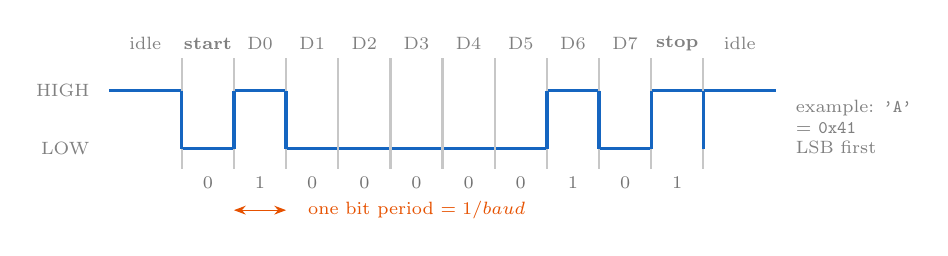
\begin{tikzpicture}[x=7.2mm, y=5mm, every node/.style={transform shape}, scale=0.92]

    % Bit pattern for 'A' = 0x41 = 0100 0001, transmitted LSB first:
    \def\bits{{0,1,0,0,0,0,0,1,0,1}}   % start, D0..D7, stop

    % Idle before and after
    \draw[very thick, draw=blkline] (-1.4,1.6) -- (0,1.6);
    \draw[very thick, draw=blkline] (10,1.6) -- (11.4,1.6);

    \foreach \i in {0,...,9}{
      \pgfmathparse{\bits[\i]}\let\lv\pgfmathresult
      \pgfmathsetmacro{\y}{\lv*1.6}
      \draw[very thick, draw=blkline] (\i,\y) -- (\i+1,\y);
      \draw[busline, draw=black!22] (\i,-0.55) -- (\i,2.5);
      \ifnum\i>0
        \pgfmathparse{\bits[\i-1]}\let\pv\pgfmathresult
        \pgfmathsetmacro{\py}{\pv*1.6}
        \draw[very thick, draw=blkline] (\i,\py) -- (\i,\y);
      \else
        \draw[very thick, draw=blkline] (0,1.6) -- (0,0);
      \fi
    }
    \draw[busline, draw=black!22] (10,-0.55) -- (10,2.5);
    \draw[very thick, draw=blkline] (10,0) -- (10,1.6);

    \node[lbl, anchor=east] at (-1.6,1.6) {HIGH};
    \node[lbl, anchor=east] at (-1.6,0)   {LOW};

    \node[lbl] at (0.5,2.9) {\textbf{start}};
    \foreach \i/\n in {1/D0,2/D1,3/D2,4/D3,5/D4,6/D5,7/D6,8/D7}{
        \node[lbl] at (\i+0.5,2.9) {\n};
    }
    \node[lbl] at (9.5,2.9) {\textbf{stop}};
    \node[lbl] at (-0.7,2.9) {idle};
    \node[lbl] at (10.7,2.9) {idle};

    \foreach \i in {0,...,9}{
      \pgfmathparse{\bits[\i]}\let\lv\pgfmathresult
      \node[lbl, text=black!55] at (\i+0.5,-0.95) {\pgfmathprintnumber{\lv}};
    }

    \draw[{Stealth[length=1.5mm]}-{Stealth[length=1.5mm]}, draw=accentline]
        (1,-1.7) -- (2,-1.7);
    \node[lbl, anchor=west, text=accentline] at (2.25,-1.7)
        {one bit period $= 1/\text{baud}$};

    \node[lbl, anchor=west, align=left] at (11.6,0.6)
        {example: \texttt{'A'}\\$=$ \texttt{0x41}\\LSB first};

    \end{tikzpicture}
    \end{center}

    \vspace{1mm}
    {\small The falling edge of the \alert{start bit} is the receiver's only timing
    reference. Data bits follow \alert{least significant bit first}.}
\end{frame}

\begin{frame}{UART or USART?}
    \leavevmode
    From here on: \alert{USART}, not UART --- that is the name of the actual
    peripheral on the STM32F446RE.

    \vspace{3mm}
    \begin{block}{The \texttt{U} stands for \emph{Universal}}
        The same hardware can also run \alert{synchronous}, with an extra clock
        pin most designs leave unconnected. Used without that pin, a USART
        behaves exactly like a plain UART --- which is how every example here
        uses it.
    \end{block}

    \vspace{2mm}
    {\small Same wire protocol, same frame, same registers below. USART is just
    the more general peripheral that happens to include UART mode.}
\end{frame}

%===============================================================================
\section{Configuring the USART}
%===============================================================================

\begin{frame}{The Registers}
    \begin{center}
    {\footnotesize
    \striped
    \begin{tabular}{@{}l l l R{.46\textwidth}@{}}
        \toprule
        \textbf{Register} & \textbf{Bit} & \textbf{Name} & \textbf{Function} \\
        \midrule
        \texttt{USART\_CR1} & 13 & \texttt{UE} & USART enable \\
                            & 12 & \texttt{M} & Word length: 0 = 8 data bits, 1 = 9 \\
                            & 10 & \texttt{PCE} & Parity control enable \\
                            & 5 & \texttt{RXNEIE} & Receive-interrupt enable \\
                            & 3 & \texttt{TE} & Transmitter enable \\
                            & 2 & \texttt{RE} & Receiver enable \\
        \midrule
        \texttt{USART\_CR2} & 13:12 & \texttt{STOP} & \phantom{}\alert{Stop bits}: 00 = 1, 10 = 2 (default: 1) \\
        \midrule
        \texttt{USART\_SR}  & 7 & \texttt{TXE} & \textbf{T}ransmit register \textbf{E}mpty --- ready for next byte \\
                            & 6 & \texttt{TC} & Transmission complete --- last bit has left the pin \\
                            & 5 & \texttt{RXNE} & \textbf{R}eceive register \textbf{N}ot \textbf{E}mpty --- a byte has arrived \\
        \midrule
        \texttt{USART\_DR}  & \multicolumn{2}{l}{7:0 (or 8:0)} & \phantom{}\alert{Data} --- write to send, read to receive \\
        \midrule
        \texttt{USART\_BRR} & \multicolumn{2}{l}{15:0} & \phantom{}\alert{Baud rate} divisor: mantissa in 15:4, fraction in 3:0 \\
        \bottomrule
    \end{tabular}}
    \end{center}

    \vspace{2mm}
    {\small On the Nucleo, \texttt{USART2} is wired to the ST-LINK and appears on
    your PC as a \alert{virtual COM port}.}
\end{frame}

\begin{frame}{Baud Rate}
	\begin{columns}[c]
		\begin{column}{.5\textwidth}
			\begin{center}
				\fbox{\parbox{.86\textwidth}{\centering\vspace{1mm}
						$\text{USARTDIV} = \dfrac{f_{\text{CK}}}{16 \times \text{baud}}$
						\vspace{1mm}}}
			\end{center}

			\vspace{3mm}
			{\small The result goes in \texttt{BRR}, with the fractional part in the
				low four bits.}
		\end{column}
		\begin{column}{.46\textwidth}
			{\small
				\striped
				\begin{tabular}{@{}l l l@{}}
					\toprule
					\textbf{Baud} & \textbf{$f_{\text{CK}}$} & \textbf{\texttt{BRR}} \\
					\midrule
					9600   & 16\,MHz & \texttt{0x0683} \\
					115200 & 16\,MHz & \texttt{0x008B} \\
					\bottomrule
			\end{tabular}}

			\vspace{3mm}
			{\small Check: $16{,}000{,}000 / (16 \times 9600) = 104.17$. The integer
				104 is \texttt{0x68}, and $0.17 \times 16 \approx 3$ --- giving
				\alert{\texttt{0x683}}.}
		\end{column}
	\end{columns}

	\vspace{3mm}
	\begin{block}{A mismatched baud rate is the classic first fault}
		Characters arrive, but as nonsense. If the very first thing you ever
		receive is garbage, suspect \alert{baud rate} before anything else.
	\end{block}
\end{frame}

\begin{frame}[fragile]{Configuring USART2}
    \begin{columns}[c]
    \begin{column}{.52\textwidth}
        \begin{lstlisting}[style=myc, basicstyle=\scriptsize\ttfamily]
void USART2_init(void) {
  // 1. Clocks: GPIOA on AHB1,
  //    USART2 on APB1
  RCC->AHB1ENR |= (1U << 0);
  RCC->APB1ENR |= (1U << 17);

  // 2. PA2/PA3 to alt. function (10)
  GPIOA->MODER &=  ~((3U<<(2*2)) | (3U<<(3*2)));
  GPIOA->MODER |=  ((2U<<(2*2)) | (2U<<(3*2)));

  // 3. AF7 (USART2), AFR[0]
  GPIOA->AFR[0] &= ~((0xFU<<(2*4)) | (0xFU<<(3*4)));
  GPIOA->AFR[0] |=  ((7U<<(2*4)) | (7U<<(3*4)));

  // 4. Baud: 9600 @ 16 MHz
  USART2->BRR = (104U << 4) | 3U;

  // 5. 8N1, enable TX and RX
  USART2->CR1 = (1U<<3) | (1U<<2);

  // 6. Enable peripheral last
  USART2->CR1 |= (1U << 13);
}
    \end{lstlisting}
    \end{column}
    \begin{column}{.44\textwidth}
        {\small Three peripheral blocks, in order: \alert{clocks}, then
        \alert{pins}, then the \alert{USART} itself. \texttt{UE} always comes
        last --- the peripheral ignores configuration changes once it is
        enabled.}

        \vspace{2mm}
        {\small This is the function every program from here on calls once,
        at the start of \texttt{main()}.}
    \end{column}
    \end{columns}
\end{frame}

\begin{frame}{TXE and RXNE: The Two Status Bits}
	\begin{center}
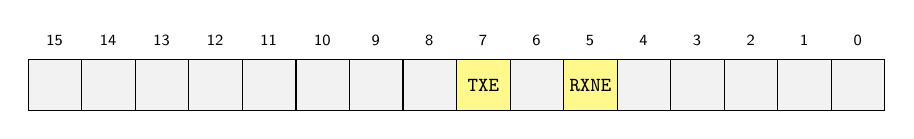
\begin{tikzpicture}[
	scale=.8,
	transform shape,
	font=\sffamily\scriptsize,
	reg/.style={
		draw,
		minimum width=8.5mm,
		minimum height=8mm,
		inner sep=0pt,
		fill=gray!10
	},
	active/.style={
		reg,
		fill=yellow!45,
		draw=black
	}
	]
	% 16-bit USART_SR layout: bits 15 down to 0
	\foreach \i in {0,...,15} {
		\pgfmathtruncatemacro{\bit}{15-\i}

		% Place bit label above the box
		\node[anchor=south] at (\i*8.5mm + 4.25mm, 1mm) {\bit};

		% Place box with TXE or RXNE inside if active bit, otherwise blank
		\ifnum\bit=7
		\node[active, anchor=north west] (b\bit) at (\i*8.5mm,0) {\small\textbf{\texttt{TXE}}};
		\else
		\ifnum\bit=5
		\node[active, anchor=north west] (b\bit) at (\i*8.5mm,0) {\small\textbf{\texttt{RXNE}}};
		\else
		\node[reg, anchor=north west] (b\bit) at (\i*8.5mm,0) {};
		\fi
		\fi
	}
	\end{tikzpicture}
	\end{center}

	\vspace{5mm}

	\begin{center}
		{\small
			\striped
			\begin{tabular}{@{}l l R{.42\textwidth}@{}}
				\toprule
				\textbf{Bit} & \textbf{Meaning} & \textbf{Used by} \\
				\midrule
				\texttt{SR} bit 7, \texttt{TXE} &
				Transmit data register empty --- safe to write \texttt{DR} &
				Program 1, every send \\

				\texttt{SR} bit 5, \texttt{RXNE} &
				Receive data register not empty --- a byte is waiting &
				Program 2, every receive \\
				\bottomrule
			\end{tabular}
		}
	\end{center}

	\vspace{2mm}

	\begin{block}{Same shape, opposite direction}
		Both programs are the same three-step pattern: \alert{initialize}, then
		\alert{wait} on one status bit, then \alert{act} in the loop body.
		\texttt{TXE} waits for room to send; \texttt{RXNE} waits for something
		to arrive. Everything else in this chapter builds on this shape.
	\end{block}
\end{frame}

\begin{frame}[fragile]{Program 1: Sending ``Hello World!''}
    \begin{columns}[c]
    \begin{column}{.52\textwidth}
        \begin{lstlisting}[style=myc, basicstyle=\footnotesize\ttfamily]
void USART2_write(int c)
{
    while (!(USART2->SR
             & (1U << 7))) ;  // wait TXE
    USART2->DR = (c & 0xFF);
}

int main(void)
{
    USART2_init();
    const char *msg = "Hello World!\r\n";
    while (*msg) {
        USART2_write(*msg++);
    }
    while (1) { }
}
    \end{lstlisting}
    \end{column}
    \begin{column}{.44\textwidth}
    \begin{center}
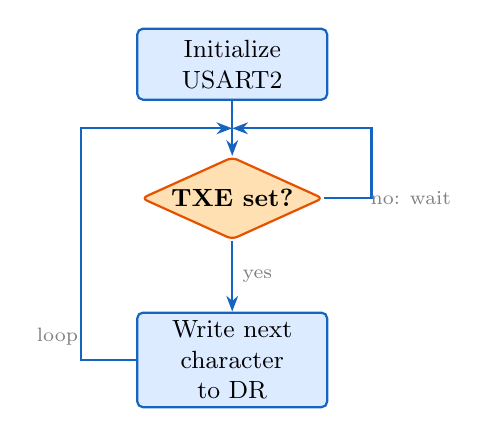
\begin{tikzpicture}[node distance=7mm, font=\sffamily\scriptsize]
	\node[blk, text width=22mm] (init) {Initialize\\USART2};
	\node[cpublk, diamond, aspect=2.2, below=of init,
	text width=16mm, inner sep=1pt] (test) {TXE set?};
	\node[blk, below=9mm of test, text width=22mm] (body)
	{Write next\\character to DR};

	% Common merge point on the incoming path
	\coordinate (merge) at ($(init.south)!0.5!(test.north)$);

	\draw[flow] (init) -- (test);
	\draw[flow] (test) -- node[lbl, right] {yes} (body);

	% Loop after writing a character
	\draw[flow] (body.west) -- ++(-7mm,0)
	|- (merge);
	\node[lbl] at ([xshift=-10mm,yshift=3mm]body.west) {loop};

	% No: wait, then rejoin the incoming path
	\draw[flow] (test.east) -- ++(6mm,0)
	|- (merge);
	\node[lbl] at ([xshift=11mm]test.east) {no: wait};
\end{tikzpicture}
    \end{center}
    {\small Each character waits for \textbf{\texttt{TXE}} (bit~7 of \texttt{SR}) before the next write --- one wait loop per byte.}
    \end{column}
    \end{columns}
\end{frame}

\begin{frame}[fragile]{Program 2: Displaying Received Characters}
    \begin{columns}[c]
    \begin{column}{.52\textwidth}
        \begin{lstlisting}[style=myc, basicstyle=\footnotesize\ttfamily]
int USART2_read(void)
{
    while (!(USART2->SR
             & (1U << 5))) ;  // wait RXNE
    return USART2->DR;
}

int main(void)
{
    USART2_init();
    while (1) {
        int c = USART2_read();
        USART2_write(c);  // show it
    }
}
    \end{lstlisting}
    \end{column}
    \begin{column}{.44\textwidth}
    \begin{center}
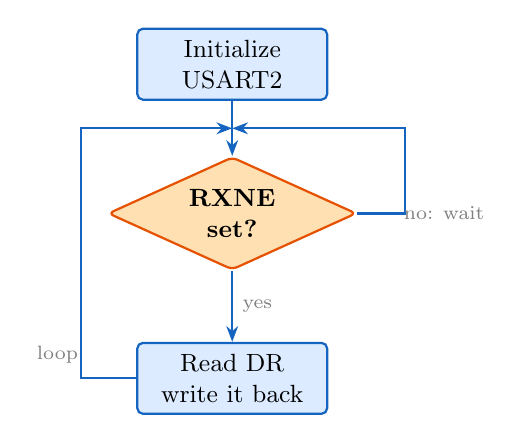
\begin{tikzpicture}[node distance=7mm, font=\sffamily\scriptsize]
	\node[blk, text width=22mm] (init) {Initialize\\USART2};
	\node[cpublk, diamond, aspect=2.2, below=of init,
	text width=16mm, inner sep=1pt] (test) {RXNE set?};
	\node[blk, below=9mm of test, text width=22mm] (body)
	{Read DR\\write it back};

	% Common merge point on the incoming path
	\coordinate (merge) at ($(init.south)!0.5!(test.north)$);

	\draw[flow] (init) -- (test);
	\draw[flow] (test) -- node[lbl, right] {yes} (body);

	% Loop after writing a character
	\draw[flow] (body.west) -- ++(-7mm,0)
	|- (merge);
	\node[lbl] at ([xshift=-10mm,yshift=3mm]body.west) {loop};

	% No: wait, then rejoin the incoming path
	\draw[flow] (test.east) -- ++(6mm,0)
	|- (merge);
	\node[lbl] at ([xshift=11mm]test.east) {no: wait};
\end{tikzpicture}
    \end{center}
    {\small Reading \texttt{DR} clears \textbf{\texttt{RXNE}} (bit~5 of \texttt{SR}) automatically --- the hardware never needs to be told explicitly.}
    \end{column}
    \end{columns}
\end{frame}

%===============================================================================
\section{UART as an Instrument}
%===============================================================================

\begin{frame}{The Most Valuable Debugging Tool You Have}
    \begin{columns}[c]
    \begin{column}{.5\textwidth}
        \textbf{What it buys you}
        \begin{itemize}
            \item See variables \alert{while the program runs}, without halting it
            \item Timestamp events and measure intervals
            \item Log a fault that happens once an hour
        \end{itemize}
    \end{column}
    \begin{column}{.46\textwidth}
        \begin{block}{What it costs}
            At 9600 baud, one character takes about \alert{1\,ms}. A 40-character
            line is \alert{40\,ms} --- which can be longer than the deadline you
            are trying to debug.
        \end{block}
    \end{column}
    \end{columns}

    \vspace{3mm}
    \begin{block}{The observer effect is real}
        Adding \texttt{printf} to a timing-sensitive routine can make the bug
        disappear --- or create a new one. Use a \alert{higher baud rate},
        \alert{shorter messages}, or set a \alert{GPIO pin} and watch it on a
        scope instead.
    \end{block}
\end{frame}

\begin{frame}[fragile]{Printing Numbers Over UART}
    \begin{columns}[c]
    \begin{column}{.56\textwidth}
        \begin{lstlisting}[style=myc, basicstyle=\scriptsize\ttfamily]
// Decimal, without printf
void uart_print_uint(uint32_t v)
{
  char buf[11]; int i = 0;
  if (v == 0) {
    uart_write('0'); return;
  }
  while (v > 0) {       // LSD first
    buf[i++] = '0' + (v % 10);
    v /= 10;
  }
  while (i > 0) {       // reverse
    uart_write((uint8_t)buf[--i]);
  }
}

// Hex -- ideal for registers
void uart_print_hex(uint32_t v)
{
  const char *d = "0123456789ABCDEF";
  uart_print("0x");
  for (int s = 28; s >= 0; s -= 4) {
    uart_write((uint8_t)d[(v>>s)&0xF]);
  }
}
    \end{lstlisting}
    \end{column}
    \begin{column}{.40\textwidth}
        {\small A few hundred bytes buy a diagnostic channel that works in
        every program from here on:}

        \begin{lstlisting}[style=myc, basicstyle=\scriptsize\ttfamily]
uart_print("MODER = ");
uart_print_hex(GPIOA->MODER);
uart_print("\r\n");
        \end{lstlisting}

        \vspace{2mm}
        {\small \alert{Avoid \texttt{printf}}: it pulls in tens of kilobytes
        and may need the heap. These cost almost nothing.}
    \end{column}
    \end{columns}
\end{frame}

\begin{frame}[fragile]{Interrupt-Driven Reception}
        \begin{lstlisting}[style=myc, basicstyle=\footnotesize\ttfamily]
volatile char     rx_buf[64];
volatile uint8_t  rx_head = 0;

void USART2_IRQHandler(void)
{
    if (USART2->SR & (1U << 5)) {        // RXNE
        rx_buf[rx_head++ & 63] = USART2->DR;   // reading DR clears RXNE
    }
}
\end{lstlisting}

    \vspace{2mm}
    \begin{block}{Why polling a UART does not scale}
        At 115200 baud a byte arrives every \alert{87\,\textmu s}. If your main
        loop takes longer than that between polls, the \alert{overrun} flag sets
        and data is \emph{lost} --- silently.

        \vspace{1mm}
        An interrupt collects each byte the moment it arrives, and
        \texttt{main()} processes the buffer when convenient.
    \end{block}
\end{frame}

\begin{frame}[fragile]{A Second Serial Link: When USART2 Is Not Enough}
    \leavevmode
    {\small Every example so far uses \texttt{USART2}, because the Nucleo's
    built-in ST-LINK makes it the easiest way to talk to a PC. But that link is
    also its limit: it is already committed. The first time a design needs a
    \alert{second} serial device --- a GPS module, a Bluetooth radio --- while
    \emph{still} printing debug output, one USART is no longer enough.}

    \vspace{2mm}
    \begin{columns}[c]
    \begin{column}{.52\textwidth}
    \begin{lstlisting}[style=myc, basicstyle=\scriptsize\ttfamily]
void USART1_init(void)
{
    RCC->AHB1ENR |= (1U << 1);  // GPIOB
    RCC->APB2ENR |= (1U << 4);  // USART1
                                 // -- APB2, not APB1
    // ... same GPIO/AF7 steps,
    // on PB6/PB7 instead of PA2/PA3
    USART1->BRR = 0x0683;
    USART1->CR1 = (1U << 3) | (1U << 2);
    USART1->CR1 |= (1U << 13);
}
    \end{lstlisting}
    \end{column}
    \begin{column}{.44\textwidth}
        {\small \texttt{USART1}, on PB6/PB7, is the natural second choice: same
        AF7 selection, same init shape. The only thing that matters
        conceptually is that \texttt{USART1} sits on \alert{APB2}, while
        \texttt{USART2} sits on \alert{APB1} --- the same $f_{\text{CK}}$
        question from the baud rate section, now relevant because the two
        peripherals no longer share a clock source.}
    \end{column}
    \end{columns}
\end{frame}

\begin{frame}{Summary}
    \begin{itemize}
        \item \textbf{Serial} sends one bit at a time --- fewer pins, longer
              distance. \textbf{Parallel} is faster but short-range.
        \item \textbf{UART is asynchronous}: no shared clock, so each byte is
              framed with a \textbf{start bit}, data (\textbf{LSB first}),
              optional parity, and a \textbf{stop bit}.
        \item Both ends must agree on \textbf{baud, data bits, parity, stop} ---
              ``9600 8N1''.
        \item $\text{USARTDIV} = f_{\text{CK}} / (16 \times \text{baud})$, written
              to \texttt{BRR}.
        \item Transmit: wait \textbf{\texttt{TXE}}, write \texttt{DR}. Receive:
              wait \textbf{\texttt{RXNE}}, read \texttt{DR}.
        \item UART is your best \textbf{diagnostic instrument} --- but printing
              takes real time, and can hide or create timing bugs.
    \end{itemize}

    \vspace{2mm}
    \begin{block}{Next: Chapter 13 --- SPI and I\textsuperscript{2}C}
        Adding a clock wire removes the speed ceiling.
    \end{block}
\end{frame}

%===============================================================================
\section{Design Challenge}
%===============================================================================

\begin{frame}{Design Challenge}{To be worked on paper, before any code}
    \leavevmode
    \begin{block}{The brief}
        Design a diagnostic protocol for the sensor monitor, to be carried over UART at 115200 baud, so that a host can observe the device without disturbing its timing.
    \end{block}

    \vspace{2mm}
    {\small Specify the message format, what is reported and how often, and how the host distinguishes a measurement from an error report. Compute the total bandwidth your protocol consumes and confirm it fits within the CPU budget. Then state which single piece of diagnostic information would be most useful to a field technician, and why you chose it over the alternatives.}
\end{frame}

\begin{frame}[plain]
    \begin{center}
        \vfill
        {\usebeamerfont{title}\color{primary}\Huge Questions?}
        \vfill
        {\small\color{Gray} \emph{Introduction to ARM Cortex-M Microprocessors} --- Chapter 12}
        \vfill
    \end{center}
\end{frame}

\end{document}

